% ! TeX root = ../../master-thesis.tex

\section{Concurrent Simulator}
\label{section:implementation:concurrent-simulator}

The implementation of a concurrent simulator is shown in the following class
diagram (Figure \ref{figure:concurrent-simulator-class-diagram}).

\begin{figure}[!ht]
  \centering
  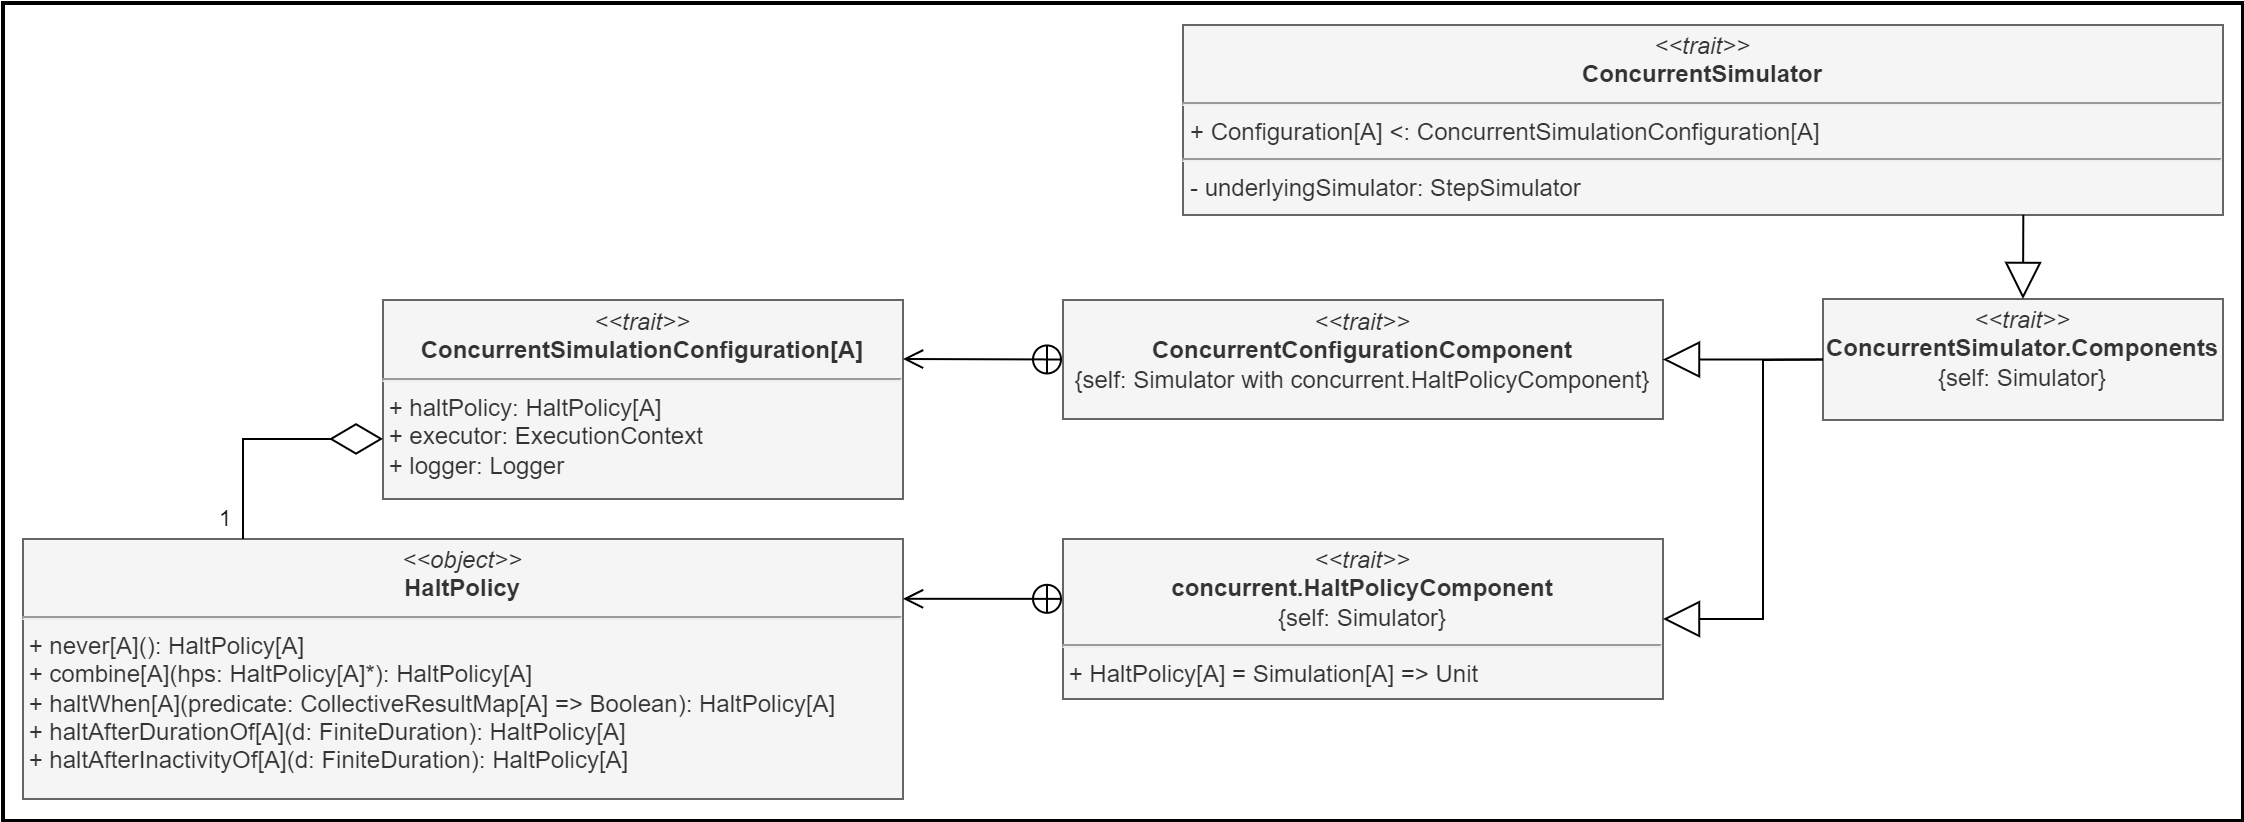
\includegraphics[width=1\textwidth]{resources/figures/concurrent-simulator-class-diagram.png}
  \caption[A UML class diagram of the concurrent simulator]{
    A UML class diagram of the concurrent simulator and its components.}
  \label{figure:concurrent-simulator-class-diagram}
\end{figure}

A \texttt{ConcurrentSimulator} is simply a \texttt{Simulator} whose
\texttt{Simulation}s are executed concurrently. A basic implementation of a
concurrent \texttt{Simulation} can be developed by leveraging an underlying
\texttt{AsyncStepSimulation}. In detail, the transmission of the device exports
to the neighbors and the user is delegated to an \texttt{ExecutionContext},
which schedules the computation on a thread pool. Transmission is scheduled as
soon as an export is generated, that is whenever the underlying simulation is
\texttt{ready}. As a consequence, from the perspective of the user, the
concurrent simulation behaves exactly the same as the base reactive model of
FRASP, without the increased observability of the step simulation, which would
have required further research to be developed due to the inherent challenges
of concurrency. Such development has been postponed since the concurrency of
the simulation did not translate to parallelism due to Sodium's transactions,
as better discussed in Section \ref{section:design:concurrent-simulation} of
the design.

The \texttt{SimulationConfiguration} of a concurrent \texttt{Simulation} is
modelled by the class \texttt{ConcurrentSimulationConfiguration}. In addition
to the \texttt{Environment} and \texttt{HaltPolicy}, the configuration includes
the \texttt{ExecutionContext} where the simulation will be executed. Some
built-in \texttt{HaltPolicy}s are already defined in the corresponding
simulator component, including \texttt{never}, \texttt{haltWhen} and two
others, namely \texttt{haltAfterDurationOf}, which halts the simulation after a
certain period of time has elapsed since its start, and
\texttt{haltAfterInactivityOf}, which halts the simulation after a certain
period of time has elapsed since its latest event.

\paragraph{Example.}
A practical application of the \texttt{ConcurrentSimulator} is demonstrated in
the following program (Listing \ref{listing:concurrent-simulator-example}).

\lstinputlisting[
  language=Scala,
  caption={
      [An application of the concurrent simulator]
      An application of \texttt{ConcurrentSimulator}. The program is very
      similar to Listing \ref{listing:step-simulator-example}, however, note
      that the concurrent simulator accepts a different configuration (line 10).
      Additionally, the exports are generated continually by the provided
      \texttt{ExecutionContext} after the simulation is started (after line 23,
      there is no \texttt{next} method to call).},
  captionpos=b,
  label={listing:concurrent-simulator-example}
]{resources/listings/concurrent-simulator-example.txt}
